\documentclass[12pt]{article}

% Language setting
% Replace `english' with e.g. `spanish' to change the document language
\usepackage[english]{babel}

% Set page size and margins
% Replace `letterpaper' with `a4paper' for UK/EU standard size
\usepackage[a4paper,top=2cm,bottom=2cm,left=2cm,right=2cm,marginparwidth=1.75cm]{geometry}

% Useful packages
\usepackage{amsmath}
\usepackage{graphicx}
\usepackage[colorlinks=true, allcolors=blue]{hyperref}
\usepackage{url}

\linespread{1.25}
\setlength{\parindent}{0px}

\title{Lecture 04}
\author{Neural Network}

\begin{document}
\maketitle{}

\section{Perceptron}
The perceptron is the simplest form of neural network. It performs binary classification that maps input features to output values in 1s and 0s. 

\begin{figure}[h]
\centering
  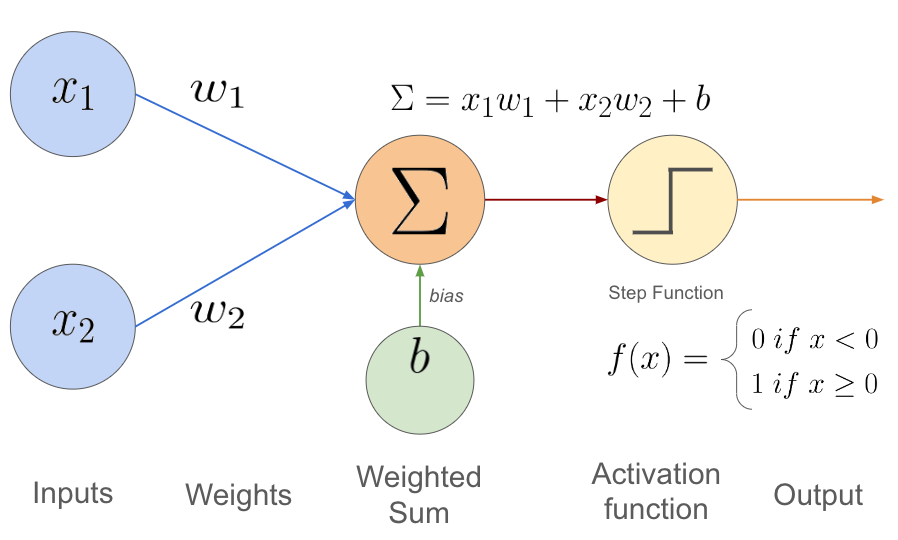
\includegraphics[width=0.5\linewidth]{images/lecture_04/img_1.png}
  \caption{Perceptron AND Gate with step function \cite{perceptronImage}}
  \label{fig:img_1}
\end{figure}

\subsection{Perceptron Problem}
Perceptrons have limitations, whereby single-layer perceptrons can only learn linearly separable patterns, which means that they can only solve problems where data can be divided by a straight line or plane. An example of the perceptron problem is the \textbf{XOR problem}.

\newpage
\section{Feed-forward Neural Network}
A feed-forward neural network consists of one or more nodes in hidden layers. Every nodes in a layer is linked to every node in the next layer, and multiple activation functions can be used in the same neural network.

\begin{figure}[h]
\centering
  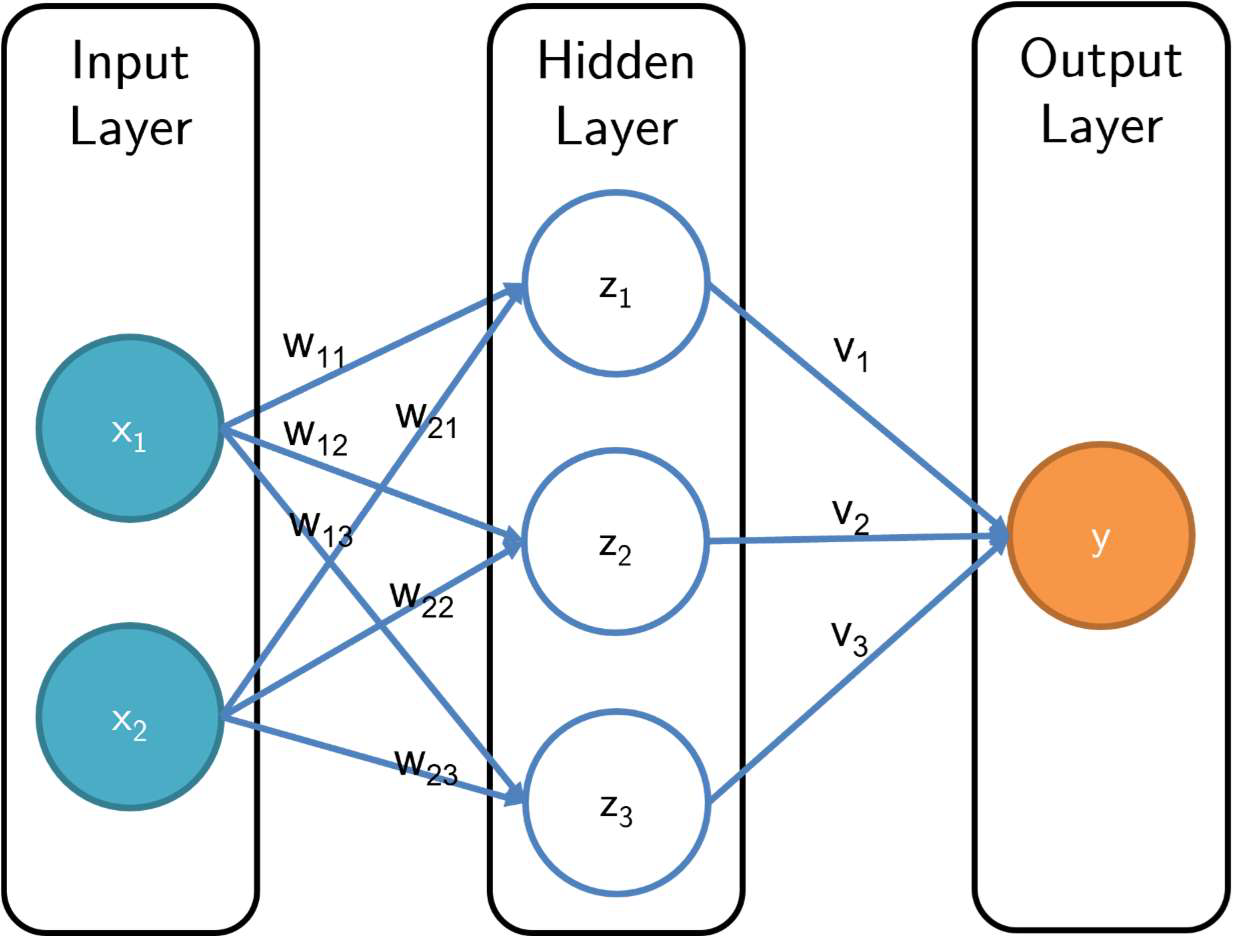
\includegraphics[width=0.5\linewidth]{images/lecture_04/img_2.png}
  \caption{Feed-forward Neural Network Diagram}
  \label{fig:img_2}
\end{figure}

\subsection{Simple Calculation of Feed-forward Neural Network}
\begin{figure}[h]
\centering
  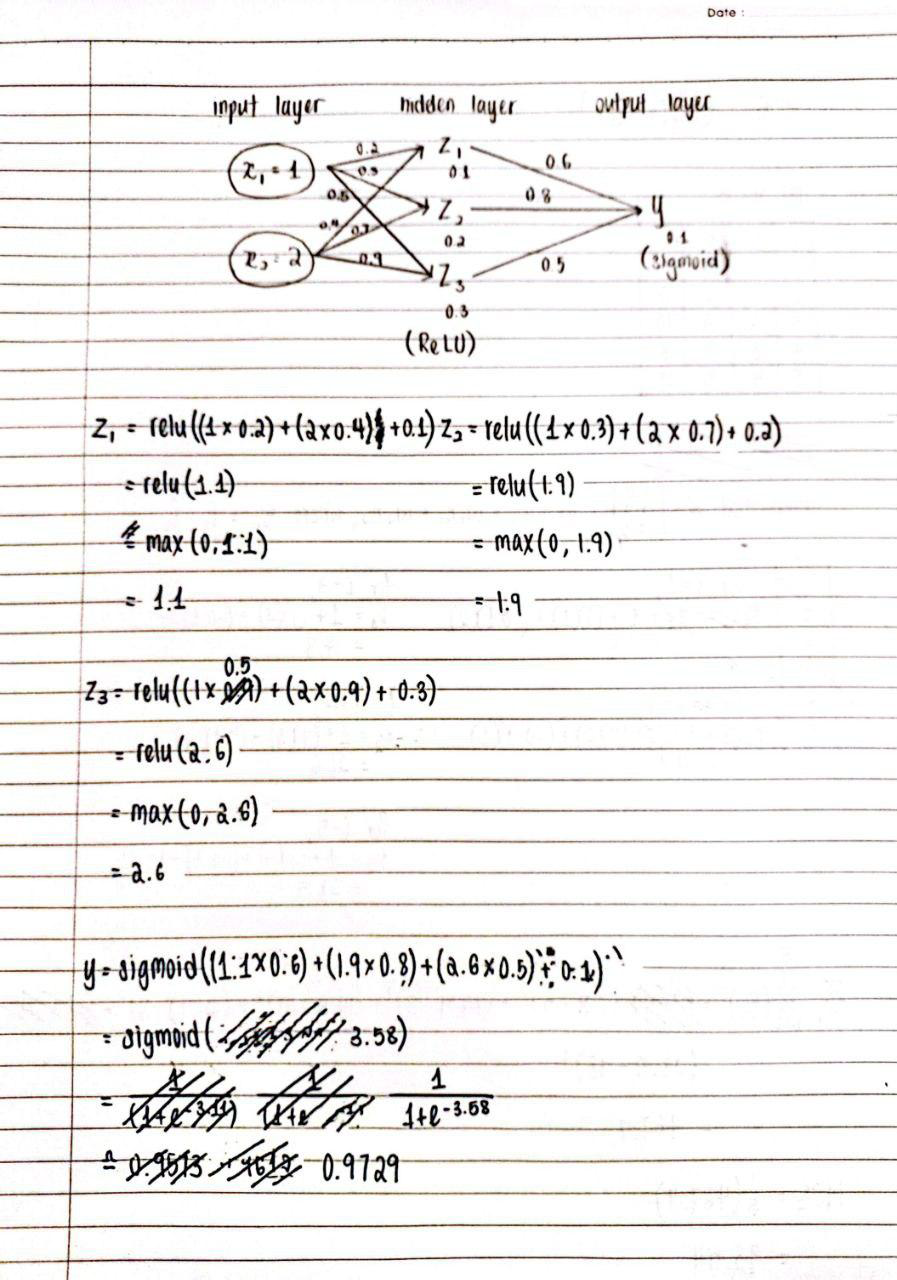
\includegraphics[width=0.475\linewidth]{images/lecture_04/img_3.png}
  \label{fig:img_3}
\end{figure}

\newpage
\section{Activation Functions}
Activation functions introduce non-linearities in neural network models, making them able to detect complex patterns from datasets. All nodes in the same neural network uses the same activation function. Let's take a look at a few of them.

\subsection{Threshold Function}
The threshold function is the simplest type of activation function. They are used in models that uses \textbf{simple logic-based}, where binary decisions are sufficient. It is rarely used in modern deep learning models.

\begin{center}
\begin{minipage}[c]{0.45\textwidth}
\[
\textit{threshold}(x) = 
\begin{cases}
1 & \text{if } x \geq 0 \\
0 & \text{if } x < 0
\end{cases}
\]
\end{minipage}
\begin{minipage}[c]{0.40\textwidth}
\centering
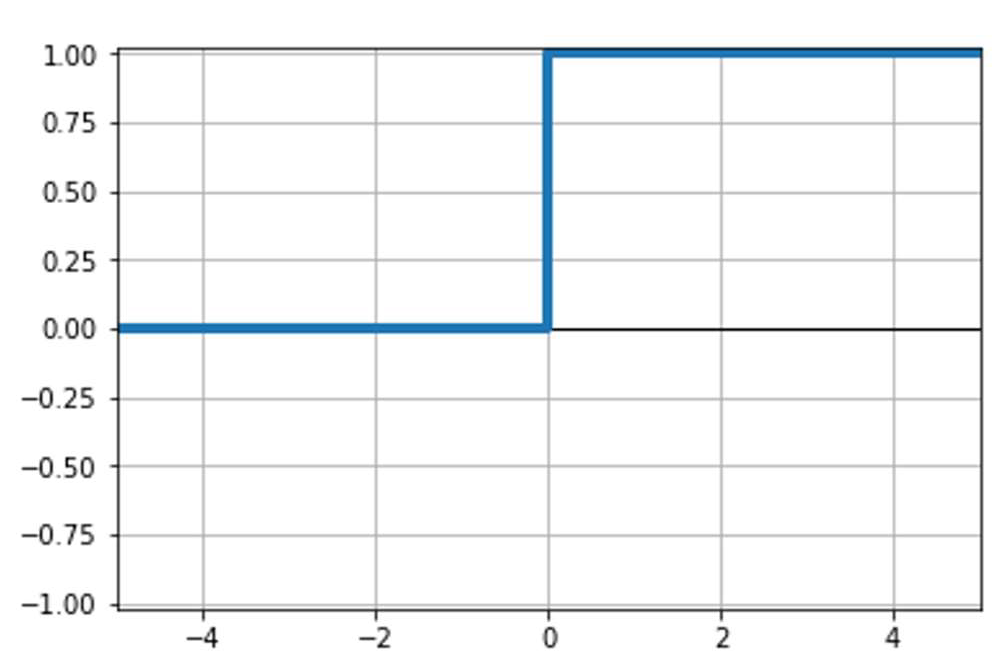
\includegraphics[width=\linewidth]{images/lecture_04/img_4.png}
\end{minipage}
\end{center}

\subsection{Sigmoid Function}
The sigmoid function is used in \textbf{binary classification problems} like logistic regression. It is suitable for neural network models where vanishing gradient is not a concern.

\begin{center}
\begin{minipage}[c]{0.45\textwidth}
\[
\textit{sigmoid}(x) = \frac{1}{1 + e^{-x}}
\]
\end{minipage}
\begin{minipage}[c]{0.40\textwidth}
\centering
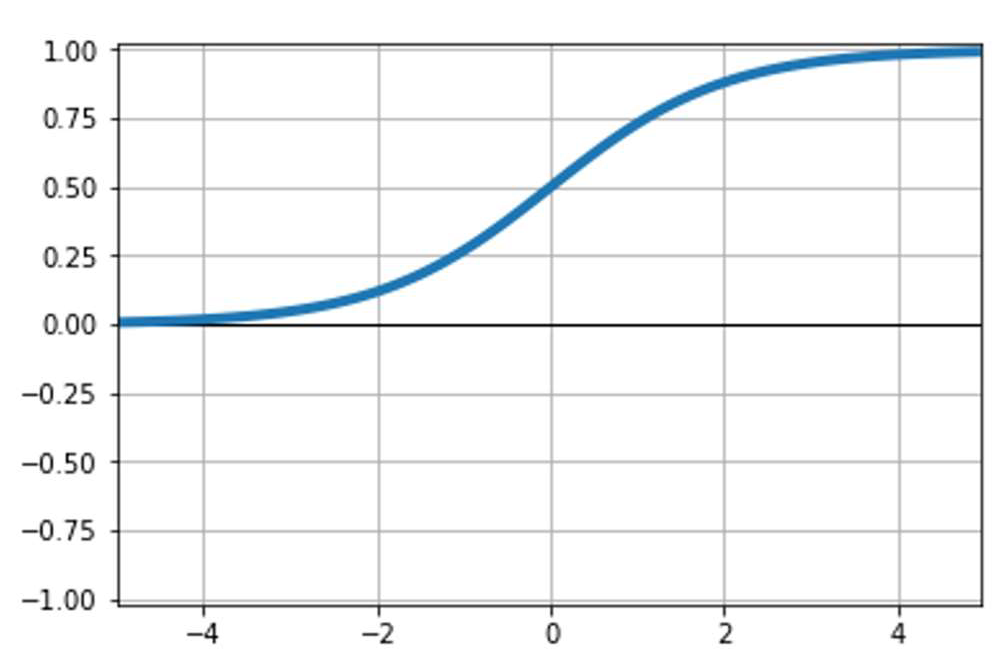
\includegraphics[width=\linewidth]{images/lecture_04/img_5.png}
\end{minipage}
\end{center}

\newpage
\subsection{Hyperbolic Tangent (tanh) Function}
The hyperbolic tangent function is used when there are zero-centered outputs (outputs in the range of -1 to 1) are present in neural network models. However, it suffers from vanishing gradients.

\begin{center}
\begin{minipage}[c]{0.45\textwidth}
\[
\textit{tanh}(x) = \frac{e^x - e^{-x}}{e^x + e^{-x}}
\]
\end{minipage}
\begin{minipage}[c]{0.40\textwidth}
\centering
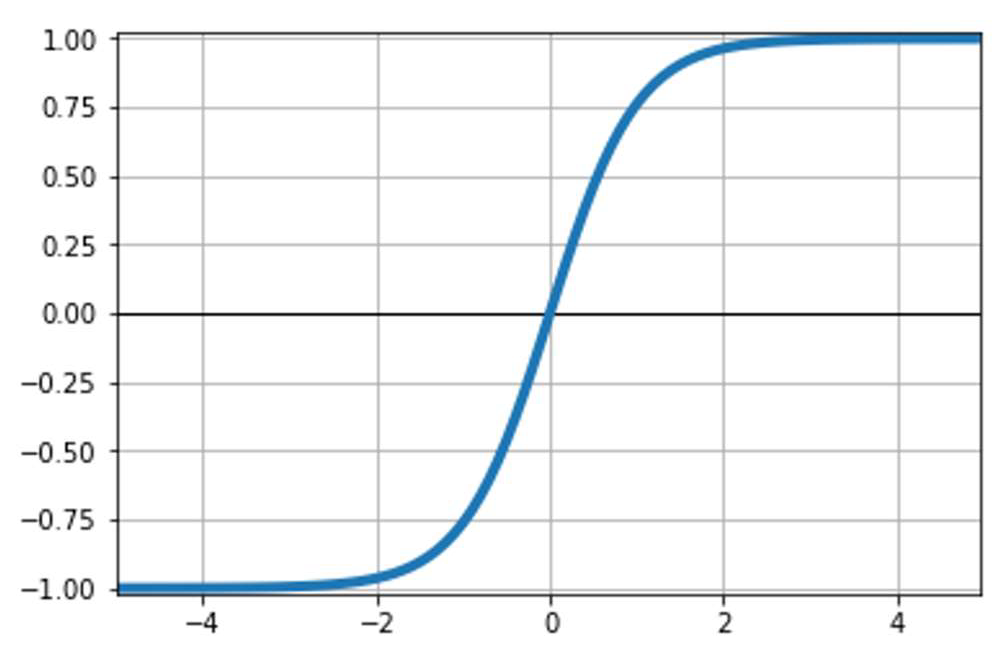
\includegraphics[width=\linewidth]{images/lecture_04/img_6.png}
\end{minipage}
\end{center}

\subsection{Rectifier Linear Unit Function}
The Rectifier Linear Unit (ReLU) function is the default choice for the hidden layers in modern deep learning models like CNNs, RNNs and transformers. This activation function enables \textbf{faster model training} and has \textbf{less vanishing gradient}.
\vspace{1.5em}

The ReLU function encourages \textbf{sparse activation}, where only a subset of neurons are only used at a time, which improves model efficiency. However, using this activation function can get neurons stuck at outputting zero if the weights become negative, this is known as the \textbf{dying ReLU problem}.

\begin{center}
\begin{minipage}[c]{0.45\textwidth}
\[
\textit{relu}(x) = \max(0, x)
\]
\end{minipage}
\begin{minipage}[c]{0.40\textwidth}
\centering
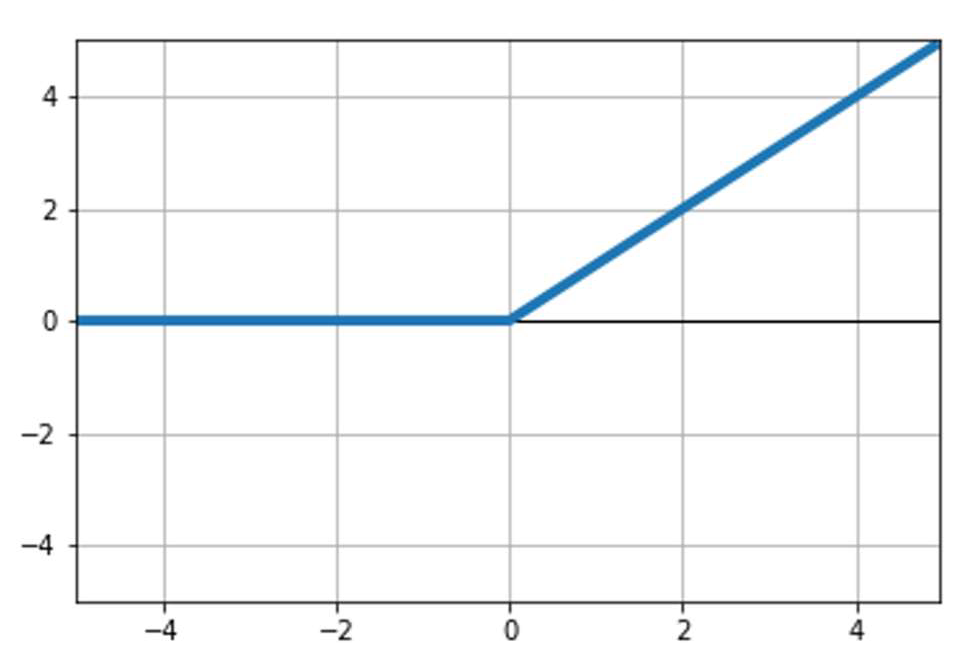
\includegraphics[width=\linewidth]{images/lecture_04/img_7.png}
\end{minipage}
\end{center}

\newpage
\section{Backpropagation in Neural Networks}
Backpropagation is the opposite of feed-forward. It involves nodes in the same neural network layer taking the error values of nodes from the subsequent layer to run the gradient descent algorithm and update their weights, that aims to minimize the loss function. The backpropagation algorithm helps neural network models to improve their accuracy and performance.
\vspace{1.5em}

The loss function used to calculate error values of the nodes depends on the type of task the neural network model is solving. Mean Squared Error will be used to solve \textbf{regression tasks} while cross-entropy will be used to solve \textbf{classification tasks}.
\vspace{1.0em}

\[
\textbf{Mean Square Error: } J = \frac{1}{N} \sum_{i=1}^{N} (y_i - \hat{y}_i)^2
\]

\[
\textbf{Cross-Entropy: } J = -\frac{1}{N} \sum_{i=1}^{N} \left( y_i \log(\hat{y}_i) + (1 - y_i)\log(1 - \hat{y}_i) \right)
\]

\subsection{Gradient Descent}
In the backpropagation section, we mentioned gradient descent. It is an optimization algorithm where the set of weight parameters converges to a point where the loss function \textit{J(w)} is minimal. 

\[
w_j = w_j - \eta \frac{\partial J}{\partial w_j}
, \quad \text{where} \quad
\frac{\partial J}{\partial w_j} = -\frac{2}{N} \sum_{i=1}^{N} (y_i - \hat{y}_i) x_{ij}
\]

\begin{figure}[h]
\centering
  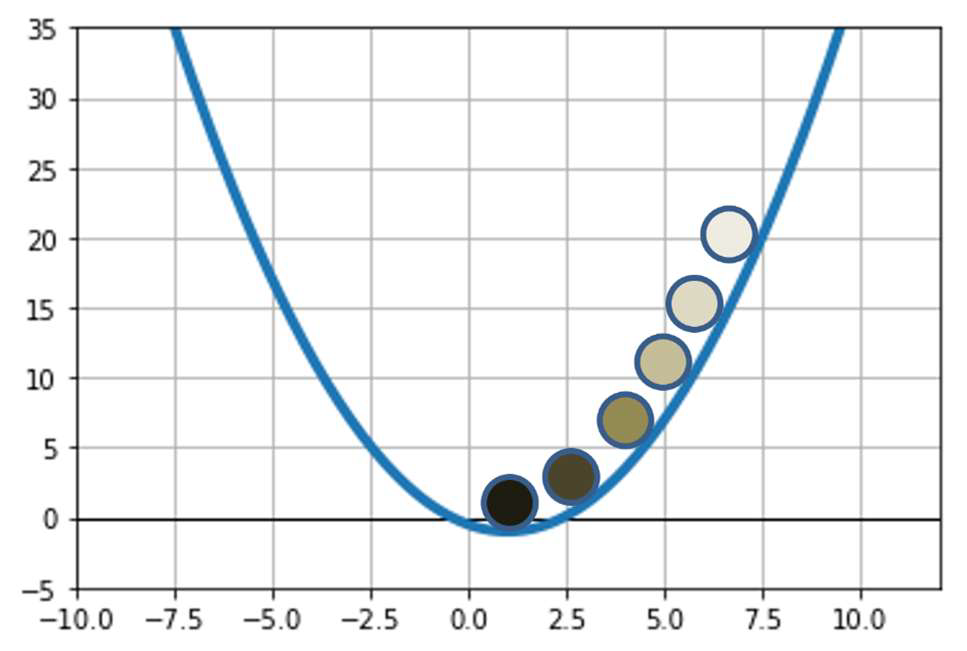
\includegraphics[width=0.475\linewidth]{images/lecture_04/img_8.png}
  \label{fig:img_8}
\end{figure}

\newpage
We can introduce learning rate $\alpha$ to the gradient descent algorithm. The learning rate allows us to control the aggressiveness of updates to the weight parameters. If the learning rate is set to too high, the gradient descent will find it hard to converge, or even diverge or oscillate. On the other hand, if the learning rate is set to too low, the gradient descent may take forever to converge, or it will be stuck at a poor local minima.
\vspace{1.5em}

A well-chosen learning rate ensures that our machine learning model is able to converge smoothly to a minimum of the loss function.

\[
w_j = w_j - \eta (\alpha) \frac{\partial J}{\partial w_j}, \quad \text{where } \alpha = \text{learning rate} 
\]

\section{Overfitting}
Overfitting occurs in machine learning models when its \textbf{training data accuracy is extremely high} while the \textbf{prediction accuracy on external datasets is low}. It indicates that the model is prone to noise after it is being trained. This phenomenon is common in deep learning models with high numbers of hidden nodes and layers.
\vspace{1.5em}

\begin{figure}[h]
\centering
  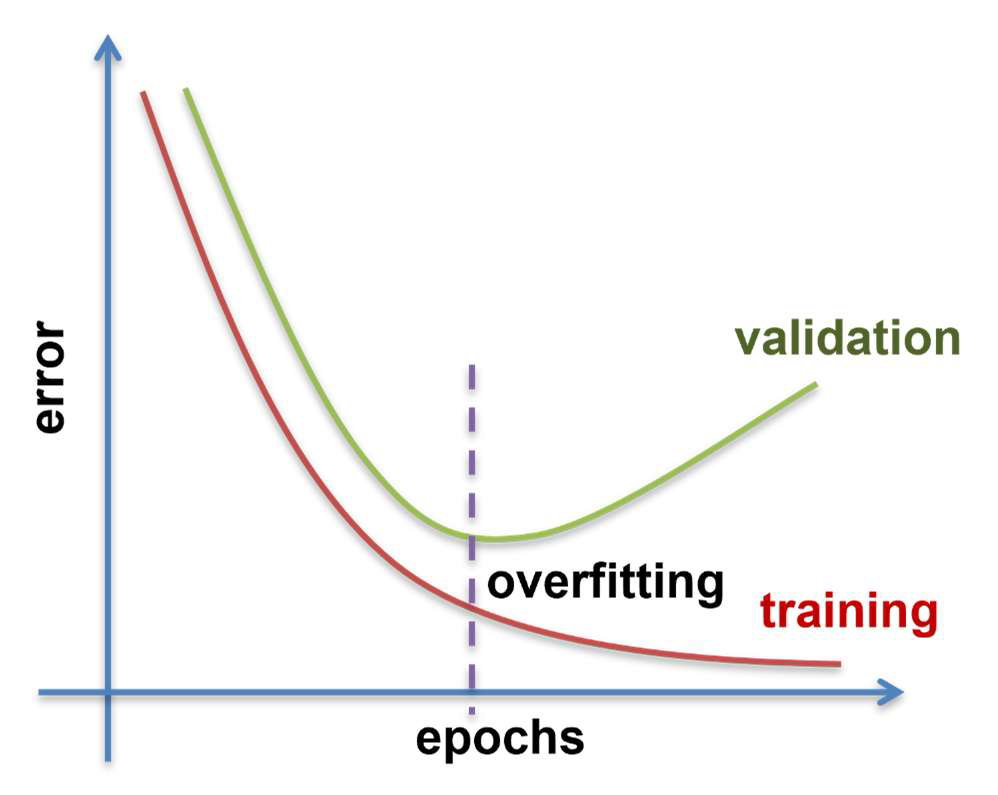
\includegraphics[width=0.475\linewidth]{images/lecture_04/img_9.png}
  \label{fig:img_9}
\end{figure}

We can overcome model overfitting by \textbf{reducing its complexity}. One way to do so is to reduce the complexity of the dataset used to train deep learning models. Principal Component Analysis is used to simplify the dataset while retaining most of the information from the dataset.
\vspace{1.5em}

Other than that, we can utilize regularization techniques like \textbf{dropout}, which randomly deactivates a subset of neurons in a neural network in every training iteration. This technique reduces dependency of neurons on other ones, to learn redundant and more robust features on their own, which makes the entire model more tolerant to variability in inputs.

\newpage
There are two other types of regularization techniques: \textbf{Lasso regularization} and \textbf{Ridge regularization}.
\vspace{1.5em}

In Lasso regularization, the sum of absolute values \textbf{(L1 norm)} of the model's weights is added to the loss function. 
\vspace{1.0em}

\[
\mathcal{L}_{\text{lasso}} = \frac{1}{N} \sum_{i=1}^{N} (y_i - \hat{y}_i)^2 + \alpha \sum_{j=1}^{M} |w_j|
\]
\vspace{1.0em}

What the regularization term $\alpha \sum_{j=1}^{M} |w_j|$ does is it encourages the model to \textbf{shrink some weights exactly to zero}, which indirectly does feature selection for us as well. Lasso regularization should be used in \textbf{sparse models}, where features are not highly correlated.


In Ridge regularization, the sum of squares \textbf{(L2 norm)} of the model's weights is added to the loss function instead.
\vspace{1.0em}

\[
\mathcal{L}_{\text{ridge}} = \frac{1}{N} \sum_{i=1}^{N} (y_i - \hat{y}_i)^2 + \alpha \sum_{j=1}^{M} w_j^2
\]
\vspace{1.0em}

What the regularization term $\alpha \sum_{j=1}^{M} w_j^2$ does is it \textbf{penalizes large weights without forcing them to zero}, which \textbf{reduces the model complexity, preventing overfitting}. Ridge regularization should be used in models with features that are highly correlated to other features, or to stabilize linear models. Unlike Lasso regularization, all model features remain in the model.
\vspace{1.5em}

We can prevent overfitting by splitting the provided datasets into training and testing datasets for model evaluation.

\newpage
\section{Cross-validation}
Cross-validation is a process in machine learning model development to choose the best performing models by comparing multiple models with different settings of hyperparameters like \textbf{number of neurons in hidden layers}, \textbf{learning rate}, and \textbf{batch size}.

\subsection{K-fold Cross-validation}
K-fold cross-validation is a commonly used type of cross-validation used in machine learning. To conduct the k-fold cross-validation, we first split our dataset into \textbf{k} equally-sized folds. In each of \textbf{k} iterations, we use \textbf{k-1} folds for training and use the remaining one for validation. We will rotate the fold used for validation in every iteration, every fold is used once for validation.

\begin{figure}[h]
\centering
  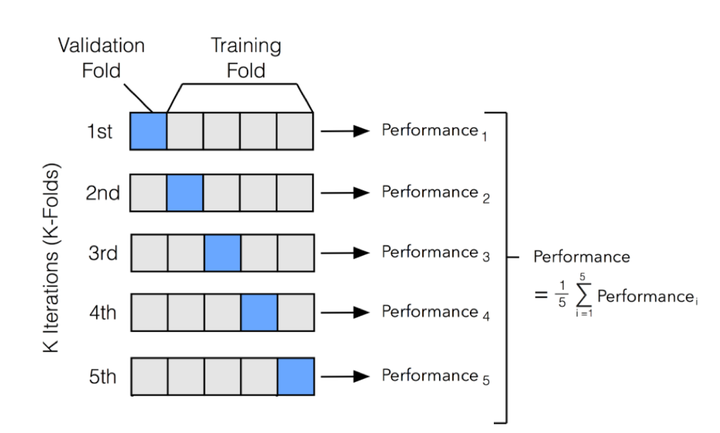
\includegraphics[width=0.60\linewidth]{images/lecture_04/img_10.png}
  \caption{\cite{crossValidationImage}}
  \label{fig:img_10}
\end{figure}

Lastly, we will average the performance metrics used (e.g., accuracy, loss, F1-score) across all \textbf{k} runs so that we get a reliable estimate of our model performance. K-fold cross-validation allows us to detect the model is overfitting when it performs well on training folds but badly on validation folds. 

\bibliographystyle{alpha}
\bibliography{bibs/lecture_04}

\end{document}